%\documentclass[compress,dvips,xcolor=table]{beamer}
\usepackage{etex}
%\documentclass{article}
%\usepackage{beamerarticle}
\usepackage{tikz}
\usetikzlibrary{positioning,arrows,matrix,calc,shapes.multipart}
%\usepackage[turkish]{babel}
\usepackage[utf8]{inputenc}
\usepackage{listings}
\usepackage{multicol}
%\includeonlyframes{current}

\def\circtxt#1{$\mathalpha \bigcirc \mkern-13mu \mathtt #1$}
\def\colorfline#1{\noalign{\color{#1} \hrule height 1pt}}
\def\colorline#1{\cr \noalign{\color{#1} \hrule height 1pt \vskip-3em}}

\mode<article>
{
  \usepackage{fullpage}
  \usepackage{pgf}
  \usepackage{hyperref}
}

\mode<presentation>
{
  \usetheme{metuceng}

%  \setbeamercovered{transparent}
}


\title{Programming Language Concepts}
\subtitle{Encapsulation}
\author{Onur Tolga Şehitoğlu}
\institute[ODTÜ]{Bilgisayar Mühendisliği}
\subject{Encapsulation}
\date{}
	\titlegraphic{\insertmetutitle\insertlicense}


\begin{document}
\lstset{language=C,
        basicstyle=\scriptsize\ttfamily,
        keywordstyle=\color{blue!50!black}\bfseries,
        identifierstyle=\color{blue!60!green}\sffamily,
        stringstyle=\color{red!70!green}\ttfamily,
	commentstyle=\color{blue!30!white}\itshape,
        showstringspaces=true}
\setbeamercolor{hexample}{bg=green!5!white,fg=black}%
\setbeamercolor{cexample}{bg=blue!5!white,fg=black}%
\setbeamercolor{pexample}{bg=orange!5!white,fg=black}%
\setbeamercolor{oexample}{bg=violet!5!white,fg=black}%

 \frame[plain]{\maketitle}
 \begin{frame}
 \frametitle{Outline}
 \begin{multicols}{2}
 \tableofcontents
 \end{multicols}
 \end{frame}

\section{Encapsulation}
\begin{frame}
\frametitle{Encapsulation}
Managing the complexity $\rightarrow$
Re-usable code and abstraction. Example:\\
\rowcolors[]{1}{blue!10}{blue!5}
\begin{tabular}{lp{.6\linewidth}}
 50 lines & no abstraction is essential, all in main() \\
 500 lines & function/procedure abstraction sufficient\\
 5,000 lines & function groups forming modules, modules are combined to form the application\\
 500,000 lines & heavy abstraction and modularization, all parts designed for reuse
 (libraries, components etc)
\end{tabular}
\end{frame}

\begin{frame}
\frametitle{Modularization and Encapsulation}
\begin{itemize}[<+->]
 \item  Building an independent and self complete set of function and variable declarations
 (\structure{Packaging})
 \item Restricting access to this set only via a set of interface function and variables.
 (\structure{Hiding and Encapsulation}) \\[2em]
\end{itemize}
\begin{tikzpicture}[private/.style = {black,thick}, public/.style = {black,thick},
		pubcall/.style = {transparent}, pubtext/.style = {transparent},pricall/.style={transparent},
		pritext/.style={transparent} ]
\only<2->{\tikzset{private/.style={red,thick}, public/.style = {green,thick}}}
\only<3-3>{\tikzset{pubcall/.style={green,draw,thick},pubtext/.style={green,fill=white},
				    pricall/.style={red,draw,thick},pritext/.style={red,fill=white}}}
\node [rectangle split, rectangle split parts=2, text width=9em,rectangle split draw splits=true] (box) {
interface 
\nodepart{two} 
detail \\
\tiny ( functions, variables, algorithm) };
\node [right of=box,xshift=5cm] (other) {other application};
\draw (box.text split west) -- (box.text split east);
\draw [private] (box.north west) -- (box.south west) -- (box.south east) -- (box.north east);
\draw [public] (box.north west) -- (box.north east);
\path [pubcall,->] (other) -- +(0,1) -| node [pubtext,pos=0.3] {$\surd$} (box.mid);
\path [pricall,->,bend left=10] (other) to  node [pritext] {$\times$} ($(box.two) +(2cm,-2mm)$);
\end{tikzpicture}
\end{frame}

\begin{frame}
\frametitle{Advantages of Encapsulation}
 \begin{itemize}
  \item High volume details reduced to interface definitions (\structure{Ease of
  development/maintenance})
  \item Many different applications use the same module via the same interface (\structure{
  Code re-usability})
  \item Lego like development of code with building blocks (\structure{Ease of
  development/maintenance}) 
  \item Even details change, applications do not change (as long as interface is kept same) (\structure{Ease of
  development/maintenance})
  \item Module can be used in following projects (\structure{Code re-usability})
 \end{itemize}

\end{frame}

\defverbatim[colored]\codenamespCpp{
\begin{lstlisting}[language={C++},escapechar=\#]
namespace Trig {
    const double pi=3.14159265358979;
    double sin(double x) { ... }
    double cos(double x) { ... }
    double tan(double x) { ... }
    double atan(double x) { ... }
   ...
};
\end{lstlisting}}
\section{Packages}
\frametitle{Packages}
\begin{frame}
\begin{itemize}
 \item A group of declarations put into a single body.
 \item C has indirect way of packaging per source file. Python defines modules per source file.
  \item C++\\
\begin{beamercolorbox}{cexample}
 \codenamespCpp
\end{beamercolorbox}
 \item \texttt{\small Trig::sin(Trig::pi/2+x)+Trig::cos(x)}
 \item C++: (\structure{::}) Scope operator.
 \item Identifier overlap is avoided. \texttt{List::insert(...)} and \texttt{Tree::insert(...)}
 no name collisions.
\end{itemize}
\end{frame}

\defverbatim[colored]\codehideH{
\begin{lstlisting}[language={Haskell},escapechar=\#]
{-- only sin, pi and cos are accessible --}
module Trig(#\color{red}{\tt sin,pi,cos}#) where
  taylorseries x = ... 
  sin x = ...
  pi=3.14159265358979
  randomseed= ...
  cos x = ...
  errorcorrect x = ...
\end{lstlisting}}
\section{Hiding}
\begin{frame}
 \frametitle{Hiding}
\begin{itemize}
 \item A group of functions and variables hidden inside. The others are interface.
Abstraction inside of a package:\\
{\scriptsize
\begin{tabular}{|>{\tt}l|} \hline
 \color{gray}double taylorseries(double);  		\\
 double sin(double x);			\\
 double pi=3.14159265358979;		\\
 \color{gray}double randomseed;	\\
 double cos(double x);			\\
 \color{gray}double errorcorrect(double x); \\ \hline
\end{tabular}}
\begin{beamercolorbox}{hexample}
 \codehideH
\end{beamercolorbox}

\end{itemize}
\end{frame}

\section{Abstract Data Types}
\begin{frame}
\frametitle{Abstract data types}
 \begin{itemize}
  \item Internals of the datatype is hidden and only interface functions provide the
  access.
  \item Example: rational numbers: 3/4 , 2/5,  19/3 \\
\texttt{data Rational = Rat (Integer,Integer) \\
x = Rat  (3,4)\\
add (Rat(a,b)) (Rat(c,d)) = Rat (a*d+b*c,b*d)} \begin{enumerate}
  \item \alert{Invalid value?}  \texttt{Rat (3,0)}
  \item \alert{Multiple representations of the same value?} \\ \texttt{Rat (2,4) = Rat (1,2)  = Rat(3,6)}
  \end{enumerate}
  \item Solution: avoid arbitrary values by the user.
 \end{itemize}
\end{frame}

\defverbatim[colored]\codeabstypeH{
\begin{lstlisting}[language={Haskell},escapechar=\#]
module Rational(#\color{red}{Rational,rat,add,subtract,multiply,divide}#) where
  data Rational = #\color{gray}{Rat}# (Integer,Integer)
  rat (x,y) = simplify (Rat(x,y))
  add (Rat(a,b)) (Rat(c,d)) = rat (a*d+b*c,b*d)  
  subtract(Rat(a,b)) (Rat(c,d)) = rat (a*d-b*c,b*d)  
  multiply(Rat(a,b)) (Rat(c,d)) = rat (a*c,b*d)
  divide (Rat(a,b)) (Rat(c,d)) = rat (a*d,b*c)
  #\color{gray}{gcd}# x y = if (x==0) then y
            else if (y==0) then x
            else if (x<y) then gcd x (y-x)
            else gcd y (x-y)
  #\color{gray}{simplify}# (Rat(x,y)) = if y==0 then error "invalid value"
                        else let a=gcd x y 
                             in Rat(div x a, div y a)
\end{lstlisting}}
\begin{frame}
Main purpose of abstract data types is to use them transparently (as if they were built-in)
without loosing \structure{data integrity}.
\begin{beamercolorbox}{hexample}
 \codeabstypeH
\end{beamercolorbox}\\
Initial value? We need \structure{constructor} function/values. (remember we don't have the
data definition)\\
\texttt {rat (x,y)}  instead of \texttt{Rat (x,y)} 
\end{frame}


 \defverbatim[colored]\codeobjcpp{
\begin{lstlisting}[language={C++},escapechar=\#]
namespace Counter {
private:   int counter=0;
public:    int get() { return counter;}
public:    void increment() { counter++; }
};
Counter::get()        Counter::increment()
\end{lstlisting}}
\section{Class and Object}
\subsection{Object}
\begin{frame}
\frametitle{Object}
 \begin{itemize}
  \item Packages containing hidden variables and access is restricted to interface functions.
  \item Variables with state
  \item Data integrity and abstraction provided by the interface functions.
  \item Entities in software can be modelled in terms of functions (server, customer record,
  	document content, etc). Object oriented design.
  \item Example (invalid syntax! imaginary C++)
\begin{beamercolorbox}{cexample}
\codeobjcpp
\end{beamercolorbox}
 \end{itemize}
\end{frame}

 \defverbatim[colored]\codeclasscpp{
\begin{lstlisting}[language={C++},escapechar=\#]
class Counter {
private:   int counter;
public:    Counter() { counter=0; }
           int get() { return counter;}
           void increment() { counter++; }
} men,vehicles;
men.increment(); vehicles.increment();
men.get(); vehicles.get();
\end{lstlisting}}
\subsection{Class}
\begin{frame}
 \frametitle{Class}
\begin{itemize}
 \item The set of same typed objects form a \structure{class}
 \item An object is an \structure{instance} of the class that it belongs to (a counter type
 instead of a single counter)
 \item Classes have similar purposes to abstract data types
 \item Some languages allows both objects and classes
 \item C++ class declaration (valid syntax):
\begin{beamercolorbox}{cexample}
\codeclasscpp
\end{beamercolorbox}
\end{itemize}
\end{frame}

\begin{frame}
\begin{columns}
 \begin{column}{.5\linewidth}
  \noindent\structure{\large Abstract data type}\\
\begin{tabular}{
!{\color{red!70!black}\vrule width 1pt}p{5cm}
!{\color{red!70!black}\vrule width 1pt}} \colorfline{green!70!black}
 interface {\tiny (constructor, functions)} \\ \hline \\
 detail {\tiny (\alert{data type definition}, auxiliary functions)}  \colorline{red!70!black} 
\end{tabular}
 \end{column}
\begin{column}{.5\linewidth}
  \noindent\structure{\large Object}\\
\begin{tabular}{
!{\color{red!70!black}\vrule width 1pt}p{4cm}
!{\color{red!70!black}\vrule width 1pt}} \colorfline{green!70!black}
 interface {\tiny (constructor, functions)}\\ \hline \\
 detail {\tiny (\alert{variables}, auxiliary functions)}  \colorline{red!70!black} 
\end{tabular}
\end{column}
\end{columns}
\ \\[2em]
\begin{block}{Purpose}
\begin{itemize}
 \item preserving data integrity, 
 \item abstraction, 
 \item re-usable codes.
\end{itemize}
\end{block}
\end{frame}

\begin{frame}
\frametitle{Further Re-usability}
\begin{itemize}
\item Class relations. Extending one class definition to create 
more specific class definitions.
\item Classes containing other classes
\item Classes derived from other classes: \structure{inheritance}
\item Abstract classes and \structure{interfaces}
\item Polymorphism
\item \structure{Design patterns:} standard object oriented designs applicable to a
	family of similar software problems. Not included in this course.
\end{itemize}
\end{frame}


\end{document}
